\documentclass[10pt]{beamer}
\usepackage{alltt}
\usepackage{graphicx}
\usepackage{xspace}
\usepackage{color}
\definecolor{linkcolor}{RGB}{16,65,69}

\newcommand{\ttt}[1]{\texttt{#1}}
\newcommand{\projname}{\ttt{bt}\xspace}

\newenvironment{monospace}{\begin{quote}\begin{alltt}}{\end{alltt}\end{quote}}

\author{Joe Colosimo \\ \small{colosimo@mit.edu} \\ Group 6}
\date{\today}


\usepackage{xmpmulti}
\usetheme{default}
\beamertemplatesolidbackgroundcolor{black}
\setbeamercolor{normal text}{fg=white}
\setbeamercolor{title}{fg=white}
\usecolortheme[named=white]{structure}
\setbeamertemplate{frametitle}[default][center]
\setbeamertemplate{navigation symbols}{}

\title{\projname}
\subtitle{A Hardware Beat Tracker}
\author{Joseph Colosimo \\ Group 6}
\date{May 15, 2013}
\institute{Massachusetts Institute of Technology}


\begin{document}
\begin{frame}
    \titlepage
\end{frame}

\begin{frame}{Tempo Estimation is Easy}
    \begin{center}
        \begin{itemize}
            \item<2-> Lots of ways to do it
            \item<3-> Lots of programs available
        \end{itemize}
    \end{center}
\end{frame}

\begin{frame}{Live Tempo Estimation is Not}
    \begin{center}
        \begin{itemize}
            \item<2-> Most methods are too resource intensive
            \item<3-> Some would would actually work with dedicated hardware
            \item<4-> I decided to try something\ldots different
        \end{itemize}
    \end{center}
\end{frame}

\begin{frame}{Architecture}
    \begin{center}
        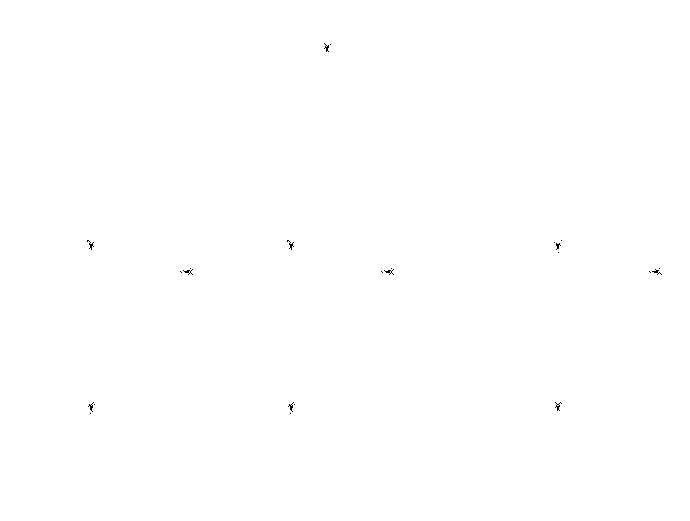
\includegraphics{fig/architecture.pdf}
    \end{center}
\end{frame}

\begin{frame}{Beat Classifier}
    \begin{center}
    \begin{align}
        \uncover<1->{S[n] &= \frac{s_l[n]^2}{2} + \frac{s_r[n]^2}{2} \\}
        \uncover<2->{e &= \frac{1}{N_L} \sum_{n=0}^{n=N_L-1} S[n] \\}
        \uncover<3->{   & (N_L \approx 1024) \\}
        \uncover<4->{\mu_E &= \frac{1}{N_E} \sum_{i=0}^{i=N_E-1} e[i] \\}
        \notag
    \end{align}

    \begin{itemize}
        \item<5-> So, keep a buffer of $e[i]$ and with each new one, subtract
                    $e[0]$ and add $e[N_E-1]$
        \item<6-> If $e > F \cdot \mu_E$, we have a beat!
        \item<7-> Choosing $F$ is hard. 1.2? 1.3? 1.4?
        \item<8-> Base it on variance: $\mu_{E^2} - \mu_E^2$
    \end{itemize}
    \end{center}
\end{frame}

\begin{frame}{Metronomes}
    \begin{center}
    \begin{itemize}
        \item<1-> KISS --- we're going to need a lot of them
        \item<2-> Need to compare themselves to received beat markings and
            output phase information
        \item<3-> Essentially, they're PLL's
        \item<4-> With each beat, halves the distance between current phase
            and new beat.
        \item<5-> $>>_{se}$ unsigned value $\Rightarrow$ free symmetric division
        \item<6-> $(16 \rightarrow 8)$    $\Leftrightarrow$ $0x10 >>_{se} 1 = 0x08$ 
        \item<7-> $(240 \rightarrow 248)$ $\Leftrightarrow$ $0xF0 >>_{se} 1 = 0xF8$ 
    \end{itemize}
    \end{center}
\end{frame}

\begin{frame}{Implementation}
    \begin{center}
        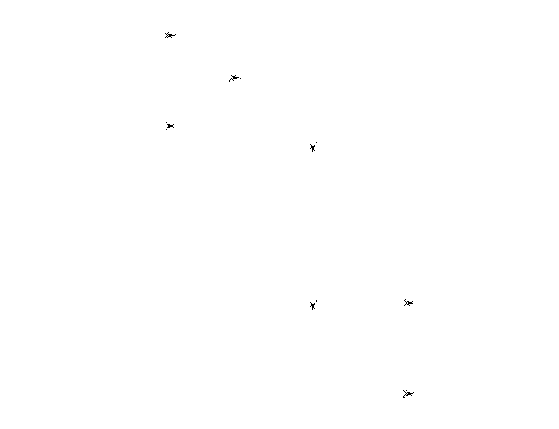
\includegraphics{fig/hwarch.pdf}
    \end{center}
\end{frame}

\begin{frame}{In Real Life}
    \begin{center}
        \includegraphics<1>{fig/dcbias.pdf}
        \includegraphics<2>[scale=0.45]{fig/dcbiasbrd.jpg}
        \includegraphics<3>[scale=0.5]{fig/setup.jpg}
    \end{center}
\end{frame}

\begin{frame}
    \begin{center}
        Let's take a look.
    \end{center}
\end{frame}


\end{document}
